\documentclass[tikz,border=10pt]{standalone}

\begin{document}
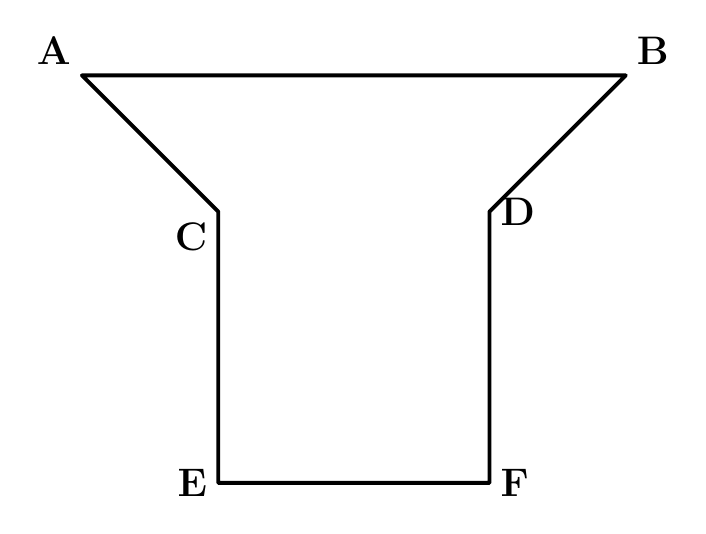
\begin{tikzpicture}[line join=round, line width=1.4pt,
  every node/.style={font=\fontsize{14.5}{17.4}\selectfont}]
\coordinate (A) at (-3.481,2.606);
\coordinate (B) at (3.426,2.606);
\coordinate (C) at (-1.749,0.875);
\coordinate (D) at (1.695,0.875);
\coordinate (F) at (1.695,-2.569);








  
  \coordinate (E) at (-1.749,-2.569);

  
  \draw (A) -- (B) -- (D) -- (F) -- (E) -- (C) -- cycle;

  
  \node[above left]  at (A) {$\mathbf{A}$};
  \node[above right] at (B) {$\mathbf{B}$};
  \node[right]       at (D) {$\mathbf{D}$};
  \node[left]        at (E) {$\mathbf{E}$};
  \node[right]       at (F) {$\mathbf{F}$};
  \node[below left]  at (C) {$\mathbf{C}$};
\end{tikzpicture}
\end{document}
